\section{Implementierung}

\subsection{GUI Komponenten}

Da die Hauptaufgabe dieser Projektarbeit darin bestand, die benötigten GUI Komponenten zu entwickeln und in richtiger Weise zusammenzusetzen, wird darauf im folgenden detailliert eingegangen.

\subsubsection{ShortcutField}

Ein ShortcutField ist -- wie in Abschnitt (XXX) bereits erwähnt -- für die Anzeige und Bearbeitung von Tastaturkürzeln zuständig. Sofern noch kein Shortcut eingegebent wurde, zeigt sie zudem eine Aufforderung zum Eingeben eines Shortcuts in Form eines Texts an (\glqq enter shortcut...\grqq). Um diesen Anforderungen gerecht zu werden, nutzt sie drei bereits bestehende Komponenten: Für das Löschen des gesamten Shortcuts dient ein CloseButton (umkreistes Kreuz), für die Anzeige und Bearbeitung des Shortcuts kommt die ShortcutView-Komponente zum Einsatz und die Textaufforderung wird durch ein JLabel realisiert.

\begin{figure}[H]
	\centering
	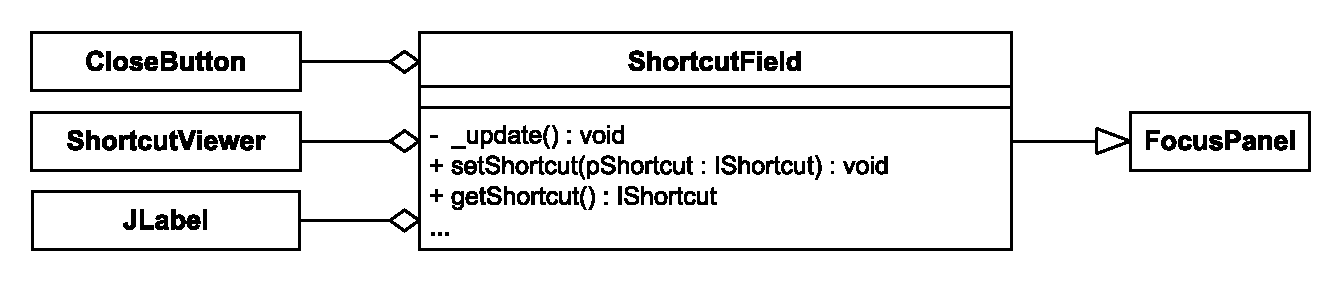
\includegraphics[width=0.8\linewidth]{../graphic/diagrams/CD_ShortcutField/ShortcutField}
	\caption{ShortcutField}
	\label{fig:shortcutfield}
\end{figure}

Die eigendliche Funktionalität wird durch die verwendeten Komponenten bereitgestellt. Selbst kümmert sich das ShortcutField um die Anzeige der jeweils richtigen Komponente (JLabel oder ShortcutView), sowie um das Horchen auf Tastatureingaben mittles eines KeyListeners. Die private Methode \_update() ist für das Ein- und Ausblenden der jeweiligen Komponente zuständig (siehe \autoref{fig:ShortcutField-update}). Sie wird initial und bei jeder Änderung des Shortcuts aufgerufen.

\begin{wrapfigure}[11]{l}[0cm]{0.50\textwidth}
    \centering
	\vspace{-5px}
	\begin{spacing}{0.75}
		\begin{javacode}[firstnumber=205]
private void _update()
{
  boolean empty = getShortcut() == null;
	
  viewerContainer.setVisible(!empty);
  textContainer.setVisible(empty);
  
  crossButton.setVisible(isEditable());
  crossButton.setEnabled(!empty);
}		\end{javacode}
	\end{spacing}
	\caption{Ein- und Ausblenden der Komponenten}
	\label{fig:ShortcutField-update}
\end{wrapfigure}

Zunächst wird überprüft, ob das ShortcutField leer ist (kein Shortcut gesetzt). Das Ergebnis dieser Überprüfung wird in der lokalen Variable empty gespeichert. Anschließend werden die Sichtbarkeiten der Komponenten aktualisiert, wobei der ShortcutViewer nur bei gesetztem und die Textaufforderung nur bei nicht gesetztem Tastenkürzel angezeigt wird. Der CloseButton wird im Editiermodus immer angezeigt aber nur aktiviert, sobald ein Shortcut eingegeben wird.

\newpage

\subsubsection{Check-Button}

Um die Grundfunktinalitäten des im Abschnitt (XXX) erwähnten Check-Buttons zu definieren, wurde zunächst das Interface ICheckComponent erstellt. Indessen wird festgelegt, dass ein Check-Button einen Checked-Zustand besitzt, welcher angibt, ob innerhalb der Komponente ein grüner Hacken (true) oder ein rotes Kreuz (false) angezeigt werden soll (siehe \autoref{fig:cdcheckbutton}).

Die Klasse CheckToggleButton implementiert das beschriebene Interface und erbt von der Swing Klasse JToggleButton. Sie kümmert sich um das Einfügen und Aktualisieren des richtigen Symbols. Innerhalb von setChecked(...) wird die private Methode \_updateIcon() aufgerufen, welche ihrerseits das jeweilige Symbol über das gesetzte Icon zeichnet (Siehe Anhang (XXX)). Insgesamt stellt ein CheckToggleButton eine vollwertige CheckComponent dar, welche direkt verwendet werden könnte.

\begin{figure}[H]
	\centering
	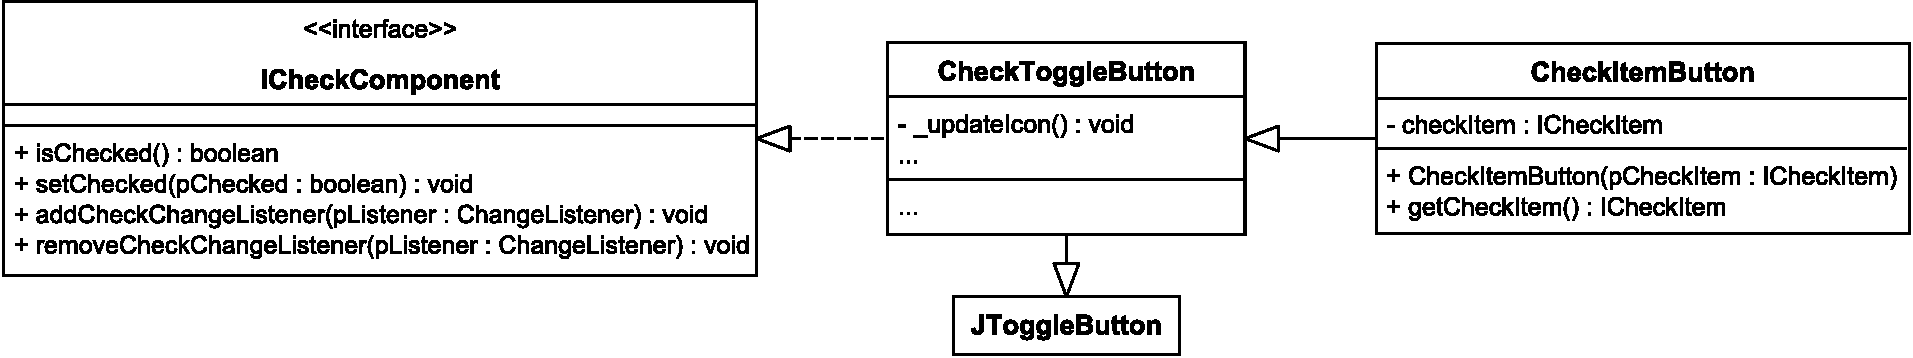
\includegraphics[width=1\linewidth]{../graphic/diagrams/CD_CheckButton/CD_CheckButton}
	\caption{CheckItemButton}
	\label{fig:cdcheckbutton}
\end{figure}

\vspace{-5px}

Um die Benutzung von CheckToggleButtons innerhalb des Shortcut Editors bzw. im Zusammenhang mit ICheckItems einfacher zu gestalten, wurde die Klasse CheckItemButton eingeführt. Diese erweitet CheckToggleButton und kann über den Konstruktor ein ICheckItem aufnehmen. Wie im Anhang (XXX) ersichtlich, werden innerhalb dieses Konstruktors alle Eigenschaften entsprechend dem ICheckItem gesetzt (z.B. Checked-Zustand oder Icon).

\vspace{-5px}

\subsubsection{CheckItemContainer}

\begin{wrapfigure}[15]{r}[0cm]{165px}
	\vspace{-12px}
	\centering
	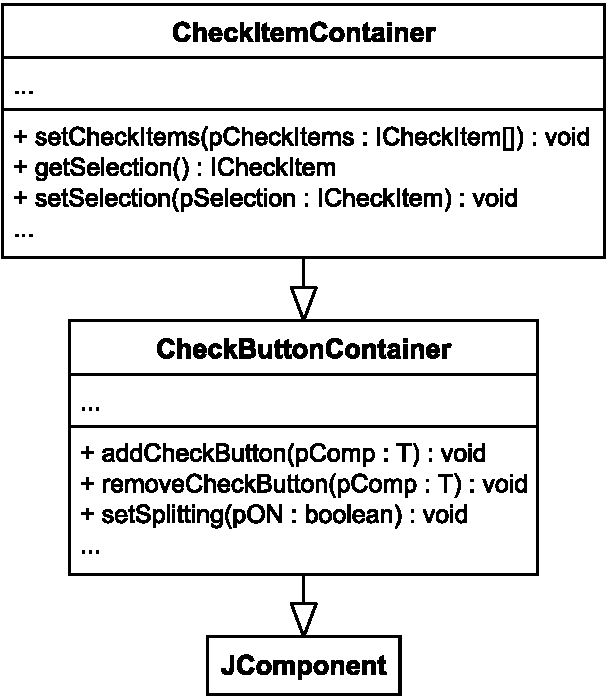
\includegraphics[width=.95\linewidth]{../graphic/diagrams/CD_CheckItemContainer/CD_CheckItemContainer}
	\caption{CheckItemContainer}
	\label{fig:cdcheckitemcontainer}
\end{wrapfigure}

Der Designentwurf lässt erkennen, dass die Check-Buttons einer bestimmten Positionierung bzw. Sortierung unterliegen: auf der linken Seite befinden sich alle unchecked und auf der rechten Seite alle checked Buttons. Zudem wird bei Browser-Check-Buttons ein Abstand zwischen den beiden Buttongruppen eingefügt. 

Um diese Positionierung zu realisieren, wurde der CheckButtonContainer erstellt. Dieser stellt eine JComponent dar, welcher mittels eines BoxLayouts seine CheckButtons horizontal nebeneinander ausrichtet. Außerdem kann der für Browser Check-Buttons erforderliche Abstand über setSplitting(...) ein- und ausgeschaltet werden. Ändert sich der Checked-Zustand eines CheckButtons, so kümmert sich der Container auch um die richtige Umsortierung.

Um wiederum die Nutzung innerhalb des Shortcut Editors zu erleichtern, existiert der CheckItemContainer. Diesem kann man CheckItems setzten (setCheckItems(...)), wonach dieser intern die benötigten Check-Buttons erzeugt und sich selbst hinzufügt oder Unnötige wieder entfernt (siehe Anhang (XXX)). Zudem kann über die Methode getSelection() der aktuell selektierte Check-Button ausgelesen werden.

\subsubsection{CheckItemAccordion}

Die Accordion-Komponente ist in der Lage, einen konkreten Pfad des Datenmodells für Browsertestergebnisse mit allen verfügbaren Details darzustellen (siehe \autoref{fig:uxDesigns}).
Jede Sektion des Accordions visualisiert also genau ein CheckItem. Sofern Untersektionen vorhanden sind, wird zusätzlich ein CheckItemContainer angezeigt. Dieser dient zur Navigation durch das Datenmodell, wobei immer genau das CheckItem dargestellt wird, welches in der vorherigen Sektion ausgewählt ist.

\begin{wrapfigure}[10]{l}[0cm]{230px}
	\vspace{-12px}
	\centering
	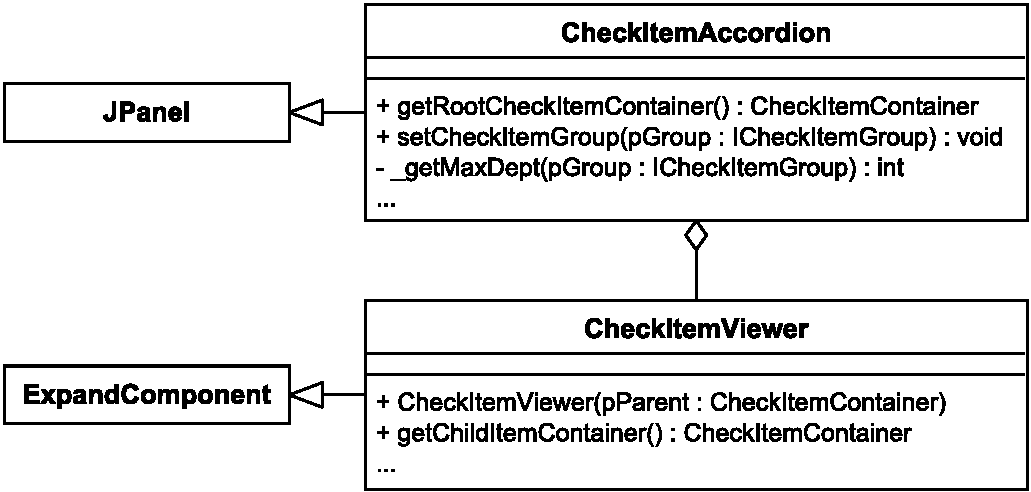
\includegraphics[width=0.95\linewidth]{../graphic/diagrams/CD_CheckItemAccordion/CheckItemAccordion}
	\caption{CheckItemAccordion}
	\label{fig:checkitemaccordion}
\end{wrapfigure}


Das CheckItemAccordion erbt von der Swing Klasse JPanel (siehe \autoref{fig:checkitemaccordion}) und verwendet zur vertikalen Positionierung der einzelnen Sektionen das BoxLayout. Im Konstruktor wird der oberste CheckItemContainer erzeugt, welcher zur Auswahl des Browsers dient und sich nicht innerhalb des Accordions befindet (siehe \autoref{fig:uxDesigns}). Um auf diesen außerhalb zugreifen zu können, dient die Methode getRootCheckItemContainer().

Eine Sektion wird durch die Klasse CheckItemViewer repräsentiert (siehe \autoref{fig:checkitemaccordion}). Diese Komponente besitzt die Fähigkeit alle Details eines CheckItems in tabellarischer Form darzustellen. Sie erbt von ExpandComponent, wodurch die Funktion des Ein- und Ausklappens und die Anzeige einer Header-Leiste ermöglicht wird. Damit das selektierte CheckItem des vorherigen CheckItemViewers angezeigt und auf Selektionsänderungen reagiert werden kann, wird im Konstruktor der vorherige CheckItemContainer übergeben. Diesem wird ein Listener hinzugefügt, welcher auf Änderungen der Selektion horcht und so die Aktualisierung des Viewers ermöglicht.

\begin{wrapfigure}[16]{r}[0px]{322px}
    \centering
	\vspace{-5px}
	\begin{spacing}{0.75}
		\begin{javacode}[firstnumber=62]
public void setCheckItemGroup(ICheckItemGroup pRootGroup)
{
  if(!Objects.equals(pRootGroup, rootGroup))
  {
    rootGroup = pRootGroup;
    
    rootCheckItemContainer.setCheckItems(pRootGroup.getItems());
    
    int dept = _getMaxDept(pRootGroup);
    CheckItemContainer children = rootCheckItemContainer;
    
    removeAll();
    for (int i = 0; i < dept; i++)
    {
      CheckItemViewer viewer = new CheckItemViewer(children);
      children = viewer.getChildItemContainer();
      add(viewer);
    }
  }
}\end{javacode}
	\end{spacing}
	\caption{Setzten der CheckItemGroup im CheckItemAccordion}
	\label{fig:CheckItemAccordion-setCheckItemGroup}
\end{wrapfigure}

In \autoref{fig:CheckItemAccordion-setCheckItemGroup} ist der Sourcecode der Methode setCheckItemGroup(...) abgebildet. In dieser wird anhand der übergebenen ICheckItemGroup das Accordion aufgebaut. Zu Beginn wird überprüft, ob es sich bei der übergebenen ICheckItemGroup um die bereits gesetzte handelt. Ist dies der Fall, so wird die Methode ohne Änderungen verlassen. Andernfalls werden dem RootCheckItemContainer die CheckItems der RootGruppe (Browser Check-Items) gesetzt. Anschließend wird über die Methode \_getMaxDept(...) die maximale Tiefe der Baumstruktur von pRootGroup ermittelt. Dieses Ergebnis dient als Grundlage für die Anzahl von Sektionen, die eingefügt werden. Nach dem Löschen aller vorhandenen Komponenten, wird in jedem Schleifendurchgang eine Sektion eingefügt. Dabei wird im Konstruktor des CheckItemViewers immer der CheckItemContainer der vorherigen Sektion oder am Anfang der rootCheckItemContainer übergeben. Dadurch wird der richtige Zusammenhang zwischen den Sektionen hergestellt.

\subsubsection{BreadCrumb und TreeTable}

Die Komponenten BreadCrumb und TreeTable mussten im Zuge dieser Projektarbeit nicht neu entwickelt werden, da sie bereits zu einem früheren Zeitpunkt umgesetz wurden. 

\begin{wrapfigure}[12]{l}[0cm]{230px}
	\vspace{-12px}
	\centering
	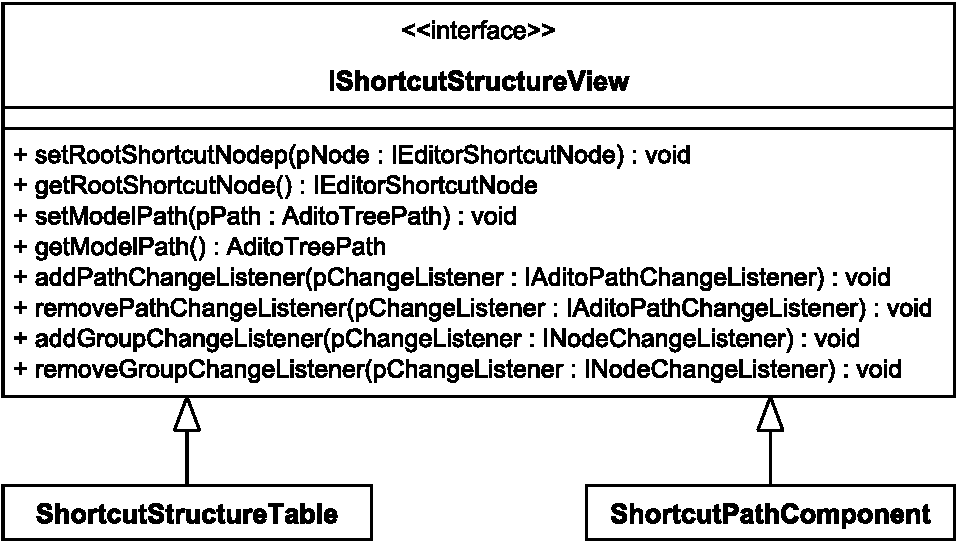
\includegraphics[width=1\linewidth]{../graphic/diagrams/CD_IShortcutStructureView/IShortcutStructureView}
	\caption{IShortcutStructureView}
	\label{fig:ishortcutstructureview}
\end{wrapfigure}

Um sie jedoch im Zusammenhang mit dem MVP-Architekturmuster verwenden zu können, mussten sie in eigene Klassen gekapselt werden, welche IShortcutStructureView (siehe \autoref{fig:ishortcutstructureview}) implementieren. Dazu wurden die Klassen ShortcutPathComponent (BreadCrumb) und ShortcutStructureTable (TreeTable) erstellt (siehe Anhang (XXX) S. (X)). Über die im Interface enthaltenen Methoden erhält die jeweilige Komponente ihre Informationen, welche zur Darstellung benötigt werden. Außerdem erhält sie die Möglichkeit Wertänderungen über Listener zu kommunizieren. Wählt der Benutzer beispielsweiße einen anderen Knoten in der BreadCrumb aus, so werden alle PathChangeListener informiert.

\subsubsection{ShortcutEditorUI}

Nach der Implementierung der einzelenen Komponenten, mussten diese zu einem gesamten User Interface zusammengesetzt werden. Hierzu wurde die Klasse ShortcutEditorUI (siehe Anhang (XXX)) erstellt. Sie implementiert das Interface IShortcutEditorUI, welches wiederum von IShortcutStructureView erbt. Zudem erbt die UI von der Swing Klasse JPanel (XXX).

\begin{figure}[H]
	\centering
	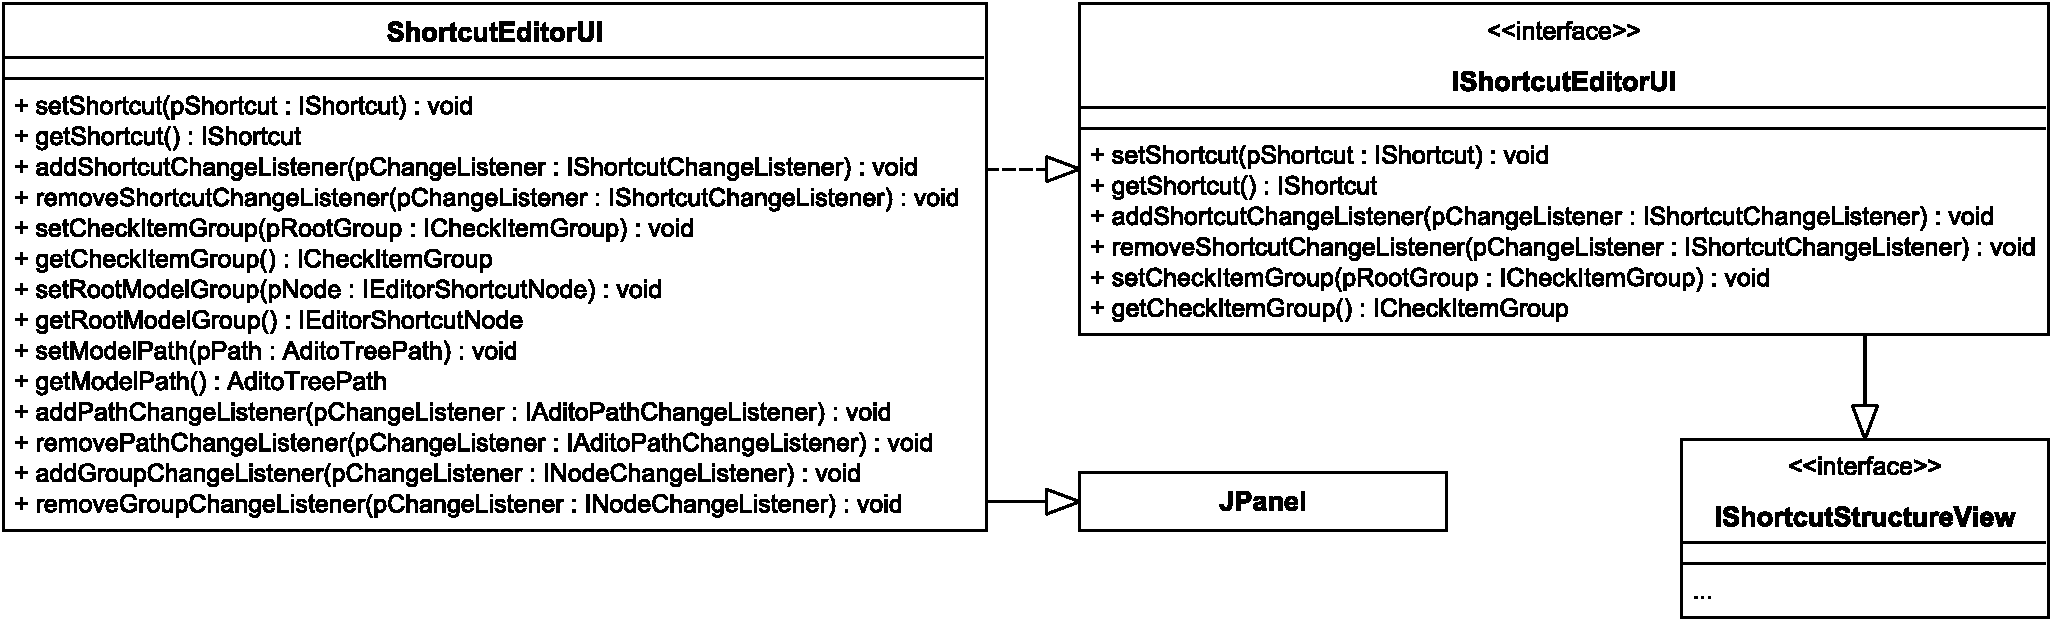
\includegraphics[width=1\linewidth]{../graphic/diagrams/CD_ShortcutEditorUI/ShortcutEditorUI}
	\caption{ShortcutEditorUI}
	\label{fig:shortcuteditorui}
\end{figure} 

\vspace{-12px}

Zur Anordnung der einzelnen Komponenten kommt das TableLayout zum Einsatz. Im Konstruktor der Klasse werden die Spalten- und Zeilenausdehnungen des Layouts definiert und die Komponenten in die entsprechenden Zellen eingefügt. Außerdem wird das ShortcutStructureModel und der ShortcutStructurePresenter initialisiert. 

Da die Funktionalität in den für die UI verwendeten Komponenten enthalten ist, werden alle Getter- und Setter-Anfragen sowie die Listener direkt an das entsprechende Element (Komponente oder Model) weitergeleitet. In der setShortcut(...) Methode der ShortcutEditorUI wird beispielsweise direkt die setShortcut(...) Methode des ShortcutFields aufgerufen und so der zu setzende Shortcut direkt weitergegeben.

\newpage

\subsection{Presenter}

Folgend wird die Implementierung des im Abschnitt (XXX) beschiebenen Presenters erläutert.

\subsubsection{ShortcutEditorPresenter}

\begin{wrapfigure}[12]{r}[0cm]{230px}
	\centering
	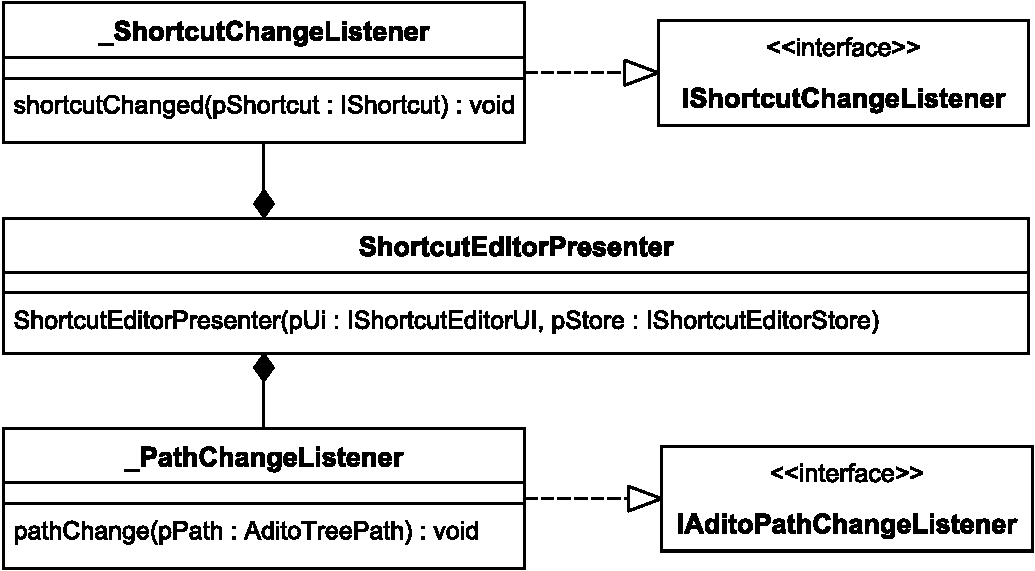
\includegraphics[width=230px]{../graphic/diagrams/CD_ShortcutEditorPresenter/ShortcutEditorPresenter}
	\caption{ShortcutEditorPresenter}
	\label{fig:shortcuteditorpresenter}
\end{wrapfigure}

Um die Daten der ShortcutEditorUI mit den in Abschnitt (XXX) beschriebenen Datenmodellen abzugleichen, existiert gemäß des MVP-Architekturmusters der ShortcutEditorPresenter (siehe Anhang (XXX) S. (X)). Diesem wird über den Konstruktor sowohl der Datenstore als auch die IShortcutEditorUI übergeben. Anschließend werden der UI Listener hinzugefügt, welche auf Shortcut- und Pfadänderungen horchen.

Ändert der Benutzer über die UI den Shortcut, so wird dieser in das entsprechende Datenmodell übertragen. Wird durch den Benutzer der Pfad geändert, also eine andere Funktion selektiert, so lädt der Presenter das Datenmodell der neuen Funktion. Zukünftige Shortcutänderungen werden dann in dieses Datenmodell übertragen.

\subsubsection{ShortcutStructurePresenter}

Da bei den beiden Komponenten TreeTable und BreadCrumb die selben Daten präsentiert werden, kommt zur Abgleichung ebenfalls das MVP-Architekturmuster zum Einsatz, wobei die beiden genannten Komponenten die Views darstellen. Der Presenter (siehe Anhang (XXX) S. (X)) erhält über den Konstruktor ein ShortcutStructureModel und eine beliebige Anzahl von IShortcutStructureViews. 

In \autoref{fig:ishortcutstructureview} wird ersichtlich, dass eine View einen IEditorShortcutNode und einen AditoTreePath besitzt. Der IEditorShortcutNode hält die in Abschnitt (XXX) beschriebene Baumstruktur der Funktionen und der Pfad gibt an, welcher Knoten des Baums gerade selektiert ist. Über Änderung dieser Attribute informieren Listener, welche der View über die entsprechenden Methoden hinzugefügt werden können (z.B. addPathChangeListener(...)). Da das ShortcutStructureModel die gleiche Funktionalität benötigt, wie die View, implementiert es auch das Interface IShortcutStructureView (siehe Anhang (XXX) S. (X)).

Im Konstruktor des ShortcutStructurePresenters (siehe Anhang (XXX) S. (X)) werden sowohl dem Model als auch den einzelnen Views Pfad- und Node-Listener hinzugefügt. Löst ein Listener des Models aus, so werden die Änderungen in alle Views übertragen. Löst ein Listener einer View aus, so werden die Änderungen in das Model übertragen. Da dadurch wiederum der Listener des Models anschlägt, werden auch die anderen Views aktualisiert. So wird gewährleistet, dass alle Views und das Model zu jedem Zeitpunkt die gleichen Informationen besitzen.

\begin{figure}[H]
	\centering
	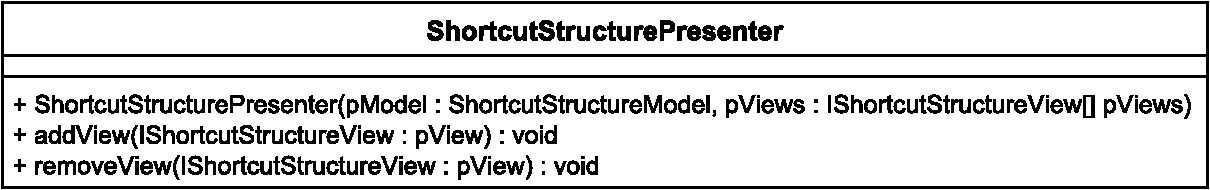
\includegraphics[width=0.6\linewidth]{../graphic/diagrams/CD_ShortcutStructurePresenter/ShortcutStructurePresenter}
	\caption{ShortcutStructurePresenter}
	\label{fig:shortcutstructurepresenter}
\end{figure}

\newpage